\documentclass[conference]{IEEEtran}
\IEEEoverridecommandlockouts
\usepackage{cite}
\usepackage{graphicx}
\usepackage{booktabs}
\usepackage{amsmath}
\usepackage{xcolor}

\begin{document}

\title{Task-Time Morphology--Motion Co-Design\\under Reconfiguration Feasibility}

\author{\IEEEauthorblockN{Anonymous Authors}
\IEEEauthorblockA{Extended abstract, IROS 2026 Workshop on Learning-based Robot Co-design}}

\maketitle

\begin{abstract}
Self-reconfigurable robots can change embodiment during a task, which creates a design decision that fixed-morphology robots never face: \emph{where can the robot physically transform?} We formulate task-time co-design over route, morphology sequence, and reconfiguration site, and ask whether modeling the physical feasibility of the transformation itself changes which design is selected. On a simulated six-pod self-mobile robot with two qualified morphologies, we compare route-first adaptation, geometry-coupled search, and feasibility-coupled search in diagnostic environments. %RESULTS-ABSTRACT%
\end{abstract}

\section{Motivation and Positioning}
Robot co-design has largely optimized a body \emph{before} deployment, from joint evolution of morphology and control~\cite{sims1994} to grammar-based and learned design search~\cite{zhao2020robogrammar,strgar2024evolution}. Self-reconfigurable modular robots instead choose embodiment \emph{during} a task. Prior work already selects configurations to satisfy task and environment requirements~\cite{jing2016smores,daudelin2018smores}, plans paths across a discrete set of morphologies~\cite{le2018htetro}, and plans module motions or connectivity changes from one configuration to another~\cite{yoshida2002,liu2019smores}. Joint morphology--navigation planning is therefore not our claim. Task-level planners commonly treat a transformation as a switch between two admissible configurations, while reconfiguration planners take the target and its location as given. The coupling between the two---two configurations can each be collision-free at a location while the module motions that connect them are not---falls between these layers.

We study this coupling as \emph{task-time iterative co-design}: embodiment is an optimization variable coupled to how and where the robot moves, over
\(\text{route} \times \text{morphology} \times \text{reconfiguration site} \times \text{transition feasibility}\).
Learned morphology search~\cite{zhao2020robogrammar,strgar2024evolution} is complementary: it expands the design space, whereas we ask whether and where an available embodiment change can physically occur within a mission.

\section{Platform and Planners}
The robot is a sensing core with six independently mobile differential-drive pods in Gazebo/ROS~2 (Fig.~\ref{fig:overview}a). Two morphologies are qualified end to end: \texttt{compact\_diff} and a longer, narrower \texttt{narrow\_tandem} for constrained passages. Reconfiguration is executed, not teleported: pods detach, drive along declared relocation paths, align using connector observations, and latch; execution tracks observed topology and inhibits assembled motion until a valid commit. The planner searches over \((x, y, \theta, m)\). Traversal edges use morphology-specific footprints and costs; transition edges carry a pre-action failure probability.

Three planners share the same mechanics, controllers, map, and disturbance realization:
\textbf{Route-first} fixes a spatial route and then inserts morphology changes along it.
\textbf{Geometry-coupled} searches route and morphology jointly, admitting a transition when a planar clearance disk and the target footprint are free.
\textbf{Feasibility-coupled} additionally samples every relocating module's 3D collision boxes along its sequential trajectory against the environment, stationary core, and support and latch conditions, and rejects the edge with a structured reason.
Thus route-first\,\(\rightarrow\)\,geometry-coupled isolates coupling route and embodiment, and geometry-coupled\,\(\rightarrow\)\,feasibility-coupled isolates physical transition feasibility.

\section{Diagnostic Study}
One passage environment is generated by shared code in three variants. The doorway admits only \texttt{narrow\_tandem}. \emph{Blocked-A} places a low post beside the attractive staging site so that before/after footprints remain admissible but the outward relocation of one pod intersects it; \emph{Blocked-B} mirrors the post to intercept a different pod; \emph{Neutral} removes it. The post lies below the lidar plane and outside the assembled robot's corridor, so it constrains only the transformation. Before simulation, deterministic planner-only checks confirmed the intended manipulation (Fig.~\ref{fig:overview}b--d). We then ran %NMISSIONS% full missions (3 variants \(\times\) 3 planners \(\times\) paired disturbance seeds) through the complete Gazebo, Nav2, localization, reconfiguration, and evaluator stack, with immutable per-trial records and provenance. Evaluator-only Gazebo poses supply clearance and contact; no planner or controller consumes them.

\begin{figure}[t]
\centering
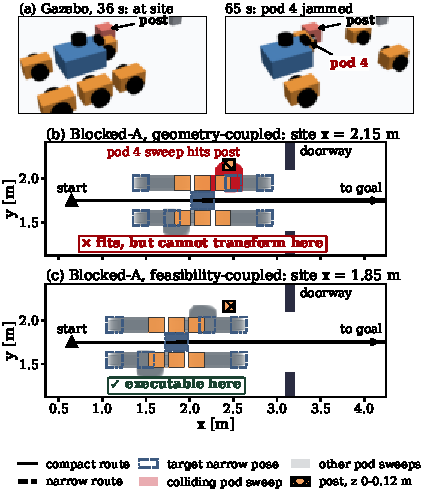
\includegraphics[width=\columnwidth]{figure_overview.pdf}
\caption{%FIGURE-CAPTION%}
\label{fig:overview}
\end{figure}

\begin{table}[t]
\caption{Preliminary diagnostic results (per variant and planner).}
\label{tab:results}
\centering
\footnotesize
%RESULTS-TABLE%
\end{table}

\section{Preliminary Results}
%RESULTS-TEXT%

\section{Discussion and Limitations}
Selecting an advantageous morphology is not sufficient when the embodiment change must happen autonomously inside the task environment: the transformation and its location become design variables. These are diagnostic cases, not a statistical comparison: two discrete morphologies, targeted simulated environments, idealized connectors and latches, and a small sample. Next steps are uncertain sensing of transition sites, learned transition-outcome models trained from executed transformations, larger morphology spaces, and hardware. Coupling generative morphology proposals with explicit transition feasibility may let robots decide not only \emph{what} to become, but \emph{when and where} they can become it.

\begin{thebibliography}{9}
\bibitem{sims1994} K. Sims, ``Evolving virtual creatures,'' in \emph{Proc. SIGGRAPH}, 1994, pp. 15--22.
\bibitem{zhao2020robogrammar} A. Zhao \emph{et al.}, ``RoboGrammar: Graph grammar for terrain-optimized robot design,'' \emph{ACM Trans. Graph.}, vol. 39, no. 6, 2020.
\bibitem{strgar2024evolution} L. Strgar, D. Matthews, T. Hummer, and S. Kriegman, ``Evolution and learning in differentiable robots,'' in \emph{Proc. RSS}, 2024.
\bibitem{jing2016smores} G. Jing, T. Tosun, M. Yim, and H. Lipson, ``An end-to-end system for accomplishing tasks with modular robots,'' in \emph{Proc. RSS}, 2016.
\bibitem{daudelin2018smores} J. Daudelin \emph{et al.}, ``An integrated system for perception-driven autonomy with modular robots,'' \emph{Science Robotics}, vol. 3, no. 23, 2018.
\bibitem{le2018htetro} A. V. Le \emph{et al.}, ``Modified A-star algorithm for efficient coverage path planning in Tetris inspired self-reconfigurable robot with integrated laser sensor,'' \emph{Sensors}, vol. 18, no. 8, 2018.
\bibitem{yoshida2002} E. Yoshida \emph{et al.}, ``A self-reconfigurable modular robot: Reconfiguration planning and experiments,'' \emph{Int. J. Robot. Res.}, vol. 21, no. 10--11, 2002.
\bibitem{liu2019smores} C. Liu, M. Whitzer, and M. Yim, ``A distributed reconfiguration planning algorithm for modular robots,'' \emph{IEEE Robot. Autom. Lett.}, vol. 4, no. 4, 2019.
\end{thebibliography}

\end{document}
